% POSTER EXAMPLE
%
% This is an example of a relatively sane poster. The box structure (and the
% narrative in general) is what I would expect, but it is completely
% non-mandatory; you may include whatever you want. Preferably, erase the
% existing box structure after you read it, and start from scratch.
%
% The main communication requirements for the poster that should be satisfied
% are as such:
%
% - At the defense, it should help you talk for around 10 minutes about your
%   thesis, and convince the committee that you did something interesting and
%   sufficiently complicated. Prepare pictures that explain your main results.
%
% - It should quickly communicate the main idea of your thesis to a random
%   educated by-walker. Ideally, a moderately-witted MFF graduate who has never
%   heard about your thesis before should be able to get the main "rough idea"
%   in less than 1 minute by just looking at the poster.

% modify the fontscale parameter to make everything slighly bigger or smaller.
\documentclass[portrait,fontscale=0.26,paperwidth=842mm,paperheight=1185mm]{baposter.cls}

\usepackage[utf8]{inputenc}
\usepackage[T1]{fontenc}

% FONT CHOICES
% Posters do not need to be PDF/A; you can choose any relatable font from the
% TeX font catalogue without much risk. Sans-serif fonts are suggested for the
% posters; see https://tug.org/FontCatalogue/sansseriffonts.html
\usepackage[sfdefault]{Fira Sans}
%\usepackage[default]{droidsans}
%\usepackage[math]{iwona}
%\usepackage[defaultfam]{montserrat}
%\usepackage{cmbright}
%\usepackage{yfonts}\renewcommand{\familydefault}{\frakdefault}

\usepackage{color}
\usepackage{graphicx}
\usepackage{amssymb,amsmath}
\usepackage[export]{adjustbox}
\usepackage{hyperref} %allows using valign with \includegraphics

\renewcommand{\arraystretch}{1.5}

\usetikzlibrary{positioning}

% A WORD ABOUT COLORS
%
% This template is prepared with a relatively neutral gray background that
% gives decent box borders (with white and darker gray), does not clash with
% many colors (except for purple-brown and other mushroomish colors, perhaps)
% and gives a lot of space for highlighting stuff.
%
% Generally, other color variations are good too; there are no strict rules on
% the colors. Good choices include:
%
% - white backgrounds and differentiation of box headers by color (see
%   headerFontColor)
%
% - various slightly tinted backgrounds (try red!10 instead of black!3)
% 
% - dark backgrounds
%
% Keep in mind:
% - The normal "informative" text and figures should be DARK on LIGHT
%   background, not the other way around.
%
% - If you want a dark background, soften (darken) the box backgrounds a bit so
%   that they do not "shine" too much from the poster. Use \color{white} for
%   the heading, and switch the UK/MFF logos to white (see contents of logos/).
%
% - Do not mix too many color hues together. Most hues have their widely
%   accepted meaning (green: good result, red: problem, blue: information,
%   yellow: highlighter, brown: serious problem, purple: something really
%   weird/interesting/magic, depending on the shade).

\begin{document}

	\color{black!80} % default font color
	\begin{poster}{grid=false,
		eyecatcher=true,
		background=plain,
		bgColorOne=white!16, % background color
		columns=2,
		headerborder=none,
		textborder=none,
		headershape=rectangle,
		headershade=plain,
		boxshade=plain,
		boxColorOne=teal!8,
		headershade=plain,
		headerColorOne=teal!24, % box header background color
		headerFontColor=black,
	}%
	{
\includegraphics[height=7em]{logos/mff-black}}
	{Autonomní křižovatka}
	{\vspace{1ex} Autor: Jiří Kotal | Vedoucí: prof. RNDr. Roman Barták, Ph.D. | 2023}
	{
\includegraphics[height=7em]{logos/uk-red}}


%
% LEFT COLUMN
%

		\begin{posterbox}[column=0,name=uvod]{1. Úvod}
			Tato práce se zabývá problémem průjezdu co největšího množství autonomních aut skrze křižovatku.
			K řešení tohoto problému používá křižovatka centrální skříňku,
			která plánuje jednotlivým autům cesty pomocí \textit{Multi-Agent Path Finding} (MAPF) algoritmů.
		\end{posterbox}

		\begin{posterbox}[column=0, name=cile, below=uvod, headerColorOne=purple!24, boxColorOne=purple!8]{2. Cíl práce}
			Cílem této práce je upravit existující MAPF řešení pro tento problém a
			následně porovnat kvalitu nalezených tras ve vytvořeném simulátoru.
			Algoritmy jsou porovnávány na různých tvarech křižovatky o různých velikostech.
			Práce zároveň zkoumá vlivy omezení tras.
		\end{posterbox}

		\begin{posterbox}[column=0, name=krizovatka, below=cile]{3. Křižovatka}
			Pro použití MAPF algoritmů, byla křižovatka převedena na orientovaný graf.
			Přči tomto převodu se rozdělí plocha křižovatky do bloků.
			Uprostřed každého bloku vznikne nový vrchol grafu, hrany se přidají mezi vrcholy sousedních bloků.
			Každý z~možných vjezdů a výjezdů je reprezentován vlastním vr\-cho\-lem.

			Tvar křižovatky je určen parametry \textit{velikost křižovatky}, \textit{počet vjezdů / výjezdů} a jejím \textit{typem}.
			\begin{itemize}
				\item Čtvercový typ křižovatky rozdělí plochu do čtvercových bloků
				\item Oktagonální typ rozšíří tuto čtvercovou mřížku o nové vrcholy reprezentující diagonální přejezdy
				\item Hexagonální typ rozdělí křižovatku se šesti stranami na~hexagonální bloky.
			\end{itemize}

			\begin{center}
				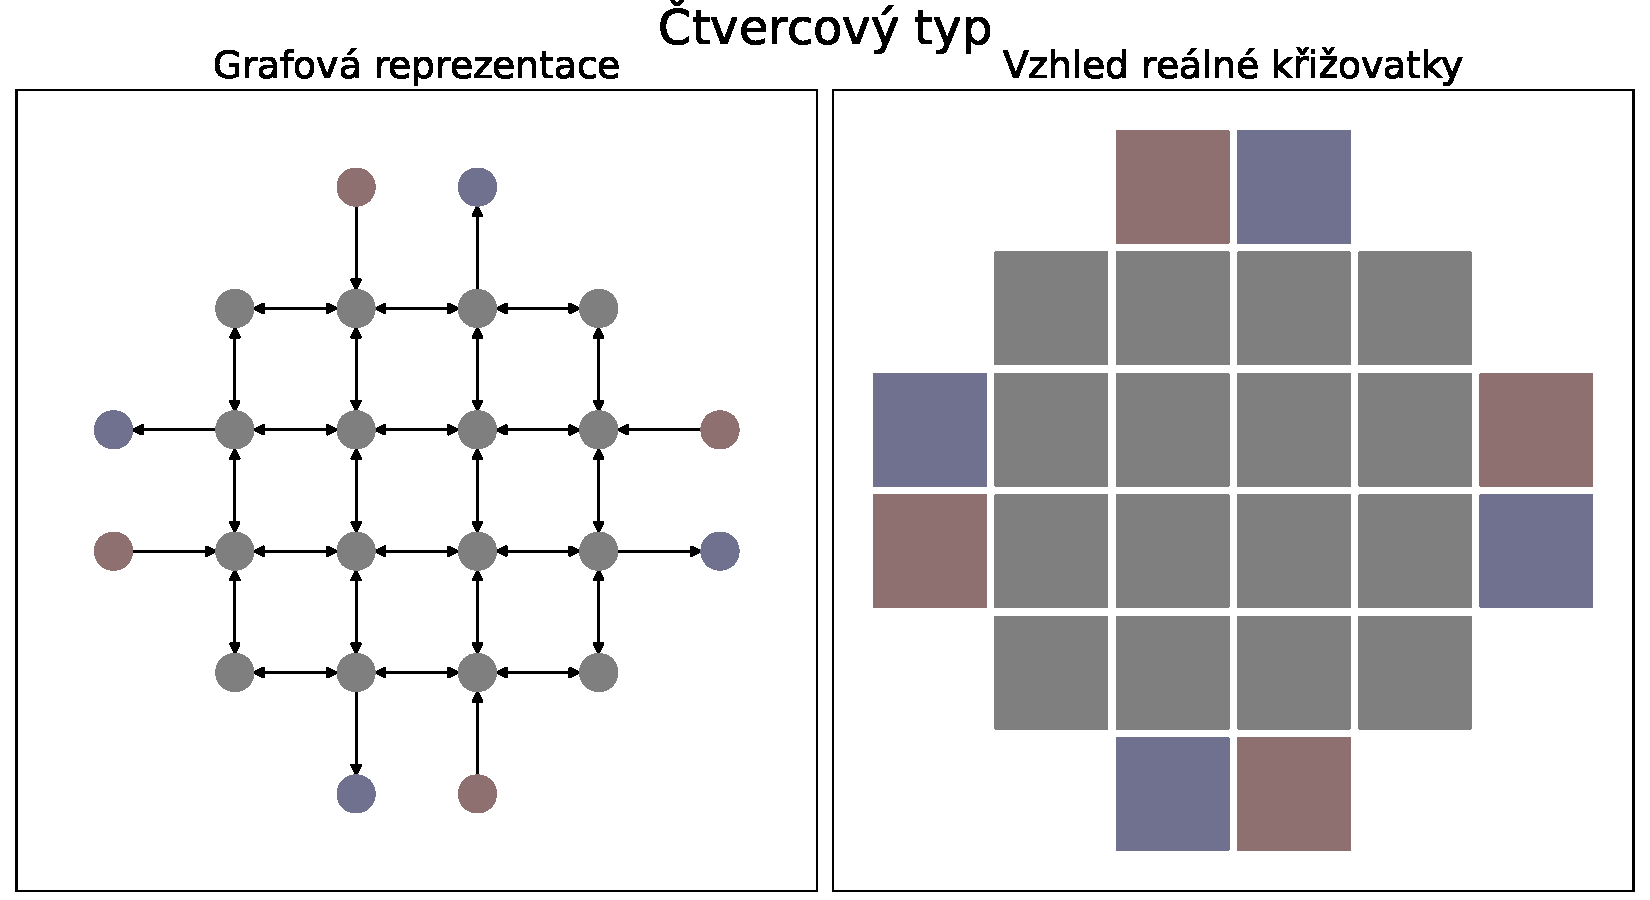
\includegraphics[width=\linewidth]{img/Square_grid}
				Ukázka křižovatky o velikosti 4 s jedním vjezdem (červená) a jedním výjezdem (modrá)
			\end{center}
		\end{posterbox}

		\begin{posterbox}[column=0, name=auto, below=krizovatka]{4. Auto}
			Autonomní auto bylo zjednodušeno na obdélník o určité velikosti.
			Je schopné jet konstantní rychlostí, nebo stát na místě.
			Auto je vždy natočené ve~směru jízdy.
			Validní trasa auta je dána posloupností vrcholů, která začíná v místě příjezdu a končí na~správném výjezdu.
			Dvě auta jsou v kolizi, pokud je průnik jejich obdélníků neprázdný.
		\end{posterbox}

		\begin{posterbox}[column=0, name=kontakt, below=auto]{8. Kontakt}
			E-mail: \href{jirikotal@vivaldi.net}{jirikotal@vivaldi.net}

			Repozitář se simulátorem: \href{https://github.com/Ji59/aim}{https://github.com/Ji59/aim}
		\end{posterbox}
%
% RIGHT COLUMN
%
% It is usually best to fill most of the poster with your results and
% conclusions. Again, use simple annotated pictures wherever possible. Plots
% with measurements are perfect, tables are also good.
%

		\begin{posterbox}[column=1, name=planovani]{5. Průběh plánování}
			Plánování je rozděleno do diskrétních kroků.
			V každém kroku jsou náhodně vygenerována nová auta a jsou přidána do fronty čekajících aut.
			Algoritmus se poté pokusí naplánovat první auta ze všech front.
			Pokud se nepovede nalézt cestu, auto čeká dál.
			Během jednoho kroku přejede auto do sousedního vrcholu podle jeho naplánované trasy.
			Pokud auto vjede na cílový vrchol, je ze simulace odstraněno.
		\end{posterbox}


		\begin{posterbox}[column=1, name=ukazka, below=planovani]{}
			\begin{center}
				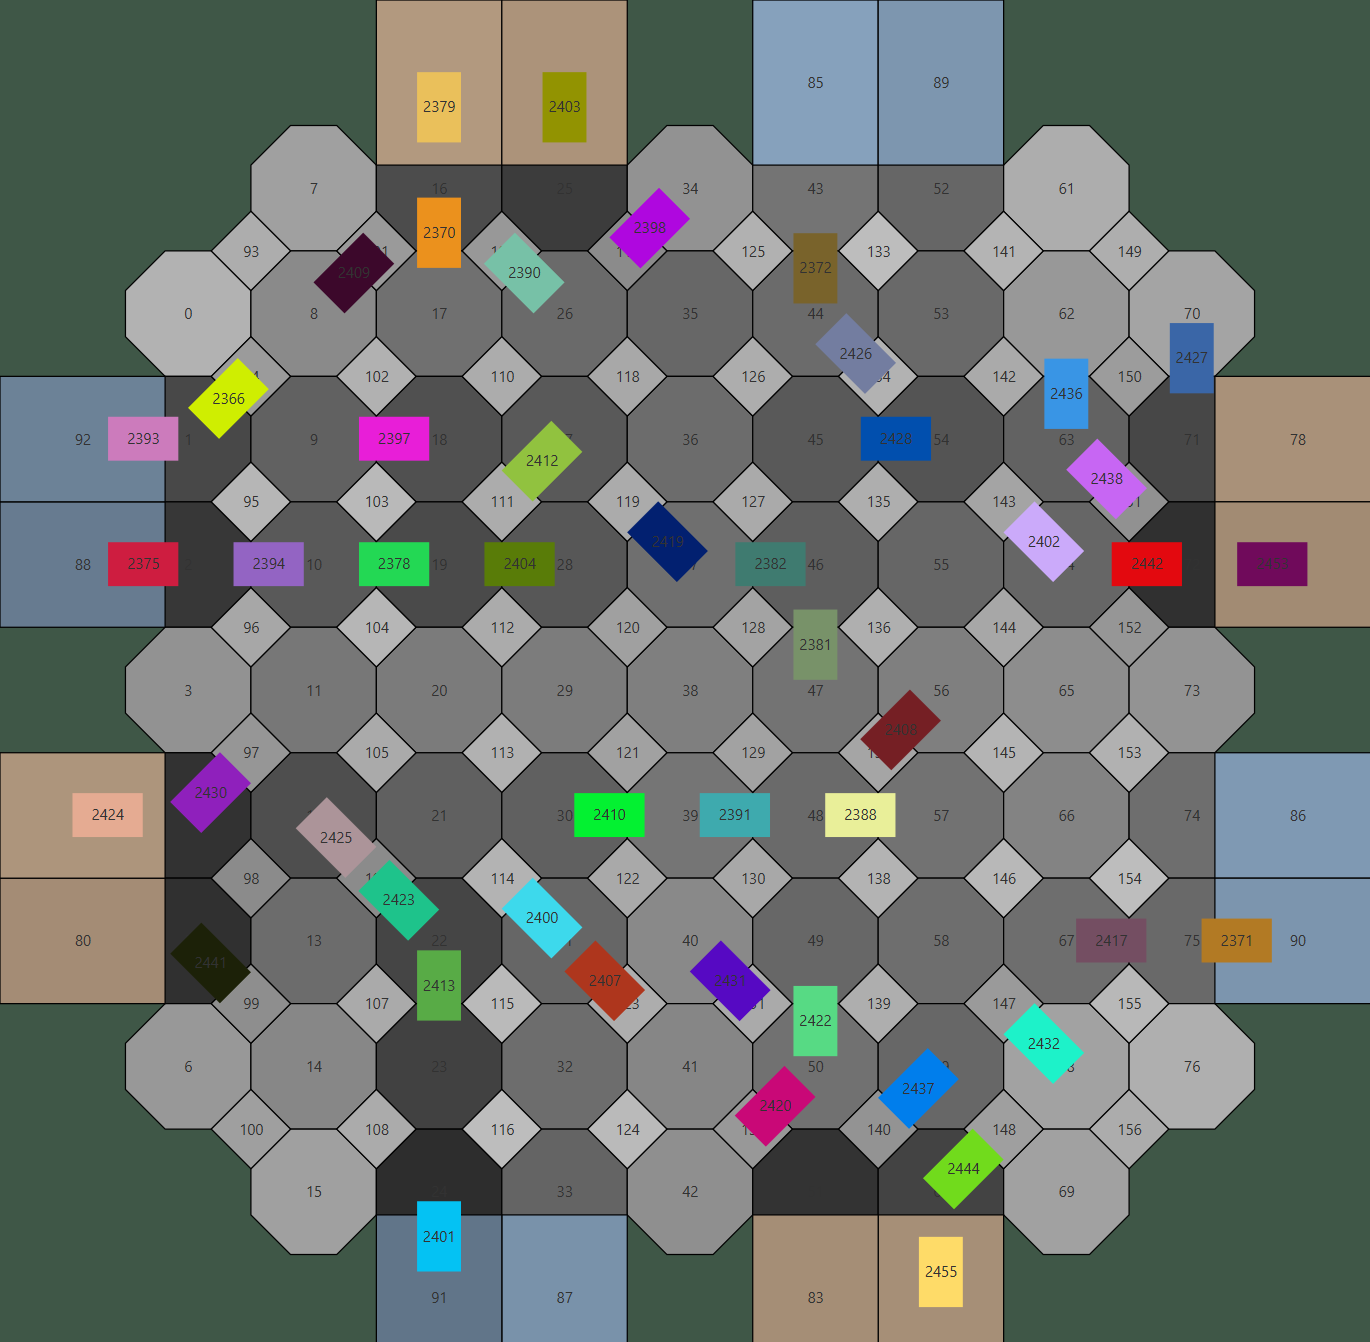
\includegraphics[width=0.79\linewidth]{img/simulator1}

				Ukázka situace ze simulátoru na oktagonální křižovatce o~velikosti 9 se 2 vjezdy a výjezdy.
			\end{center}
		\end{posterbox}

		\begin{posterbox}[column=1, name=algoritmy, below=ukazka]{6. Algoritmy}
			Jsou základní 3 varianty algoritmů podle způsobu plánování:
			\begin{itemize}
				\item Sekvenční plánování jednoho auta po druhém
				\item Plánování všech nových aut z daného kroku
				\item Přeplánování jedoucích aut společně s novými auty
			\end{itemize}

			Implementované algoritmy:
			\begin{itemize}
				\item \textit{Safe Lanes} - základní algoritmus pro porovnání
				\item \textit{A*} - implementován ve všech třech variantách
				\item \textit{Conflict-Based Search} (CBS) - rozšíření A*
				\item \textit{SAT} - předvedení na MAX-SAT
			\end{itemize}

			Všechny algoritmy mají nastavitelné parametry, např.
			maximální délka trasy auta, povolení pro auta stát na místě, \dots
		\end{posterbox}

		\begin{posterbox}[column=1, name=vysledky, below=algoritmy, headerColorOne=purple!24, boxColorOne=purple!8]{7. Výsledky}
			Při běhu byl sledován počet zamítnutých aut, prodleva aut a čas plánování.

			Měření ukázala, že neexistuje jediné nejlepší řešení a ani ideální nastavení parametrů.
			Výsledky byly závislé na typu a velikosti křižovatky.
			První varianta A* dává rychle dobré výsledky.
			Zbylé varianty A* byly velmi paměťově náročné.
			CBS se choval na~menších křižovatkách velmi dobře.
			SAT algoritmy měly dlouhé časy plánování,
			avšak jako jediné plánovaly rychleji na~plnějších křižovatkách.
		\end{posterbox}
	\end{poster}
\end{document}
